%------------------------------------------------------------


\begin{frame}
\frametitle{Why}
\begin{columns}[c] % The "c" option specifies centered vertical alignment while the "t" option is used for top vertical alignment

\column{.4\textwidth} % Left column and width
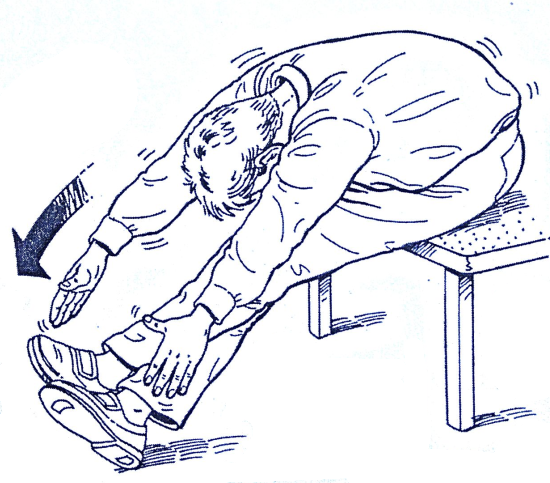
\includegraphics[width=\linewidth]{Gravity_Glider.png}
\column{.6\textwidth} % Right column and width
When the muscles of the hip (Iliopsoas muscles) are too tense as a reaction of prolonged sitting, mobility, elasticity and the even flow of blood and lymph gets disturbed. The relaxation of this muscle group is important for the equilibrium and the coordination of the whole body. Furthermore, this muscle group affects the capacity of understanding.

The gravity glider relaxes this muscle group.
\end{columns}
\end{frame}
%------------------------------------------------------------
%------------------------------------------------------------
\begin{frame}
\frametitle{How}
\begin{columns}[c]
\column{.4\textwidth} % Left column and width
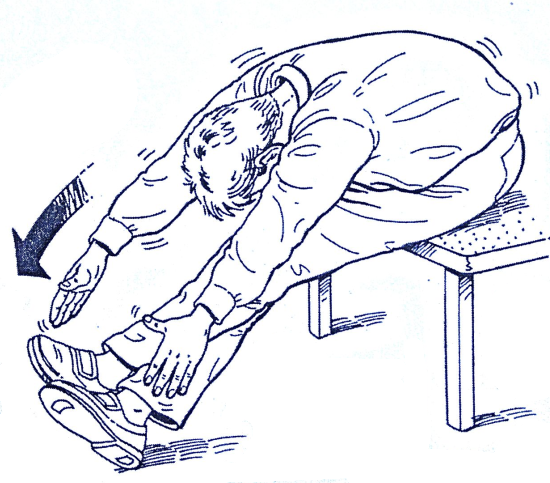
\includegraphics[width=\linewidth]{Gravity_Glider.png}
\column{.6\textwidth} % Right column and width
Sit comfortably on a chair. Put one ankle on top of the other and keep your knees slightly flexed. Exhale slowly, in the meanwhile bend forward with the head down. Stretch your arms and let them glide forward, parallel to the legs, as far as is comfortable for you.

While inhaling glide back into the upright position, at the very end pull your head up. Repeat for three or more breath cycles.

Then change your legs and repeat the sequence.
\end{columns}

\vspace{1cm}
Back to \href{run:./Exercises.pdf}{\underline{exercises}}.
\end{frame}
%------------------------------------------------------------
